% Options for packages loaded elsewhere
\PassOptionsToPackage{unicode}{hyperref}
\PassOptionsToPackage{hyphens}{url}
%
\documentclass[
]{book}
\usepackage{amsmath,amssymb}
\usepackage{lmodern}
\usepackage{ifxetex,ifluatex}
\ifnum 0\ifxetex 1\fi\ifluatex 1\fi=0 % if pdftex
  \usepackage[T1]{fontenc}
  \usepackage[utf8]{inputenc}
  \usepackage{textcomp} % provide euro and other symbols
\else % if luatex or xetex
  \usepackage{unicode-math}
  \defaultfontfeatures{Scale=MatchLowercase}
  \defaultfontfeatures[\rmfamily]{Ligatures=TeX,Scale=1}
\fi
% Use upquote if available, for straight quotes in verbatim environments
\IfFileExists{upquote.sty}{\usepackage{upquote}}{}
\IfFileExists{microtype.sty}{% use microtype if available
  \usepackage[]{microtype}
  \UseMicrotypeSet[protrusion]{basicmath} % disable protrusion for tt fonts
}{}
\makeatletter
\@ifundefined{KOMAClassName}{% if non-KOMA class
  \IfFileExists{parskip.sty}{%
    \usepackage{parskip}
  }{% else
    \setlength{\parindent}{0pt}
    \setlength{\parskip}{6pt plus 2pt minus 1pt}}
}{% if KOMA class
  \KOMAoptions{parskip=half}}
\makeatother
\usepackage{xcolor}
\IfFileExists{xurl.sty}{\usepackage{xurl}}{} % add URL line breaks if available
\IfFileExists{bookmark.sty}{\usepackage{bookmark}}{\usepackage{hyperref}}
\hypersetup{
  pdftitle={Gridded GDP projections compatible with the five SSPs},
  pdfauthor={Daisuke Murakami, Takahiro Yoshida, Yoshiki Yamagata},
  hidelinks,
  pdfcreator={LaTeX via pandoc}}
\urlstyle{same} % disable monospaced font for URLs
\usepackage{longtable,booktabs,array}
\usepackage{calc} % for calculating minipage widths
% Correct order of tables after \paragraph or \subparagraph
\usepackage{etoolbox}
\makeatletter
\patchcmd\longtable{\par}{\if@noskipsec\mbox{}\fi\par}{}{}
\makeatother
% Allow footnotes in longtable head/foot
\IfFileExists{footnotehyper.sty}{\usepackage{footnotehyper}}{\usepackage{footnote}}
\makesavenoteenv{longtable}
\usepackage{graphicx}
\makeatletter
\def\maxwidth{\ifdim\Gin@nat@width>\linewidth\linewidth\else\Gin@nat@width\fi}
\def\maxheight{\ifdim\Gin@nat@height>\textheight\textheight\else\Gin@nat@height\fi}
\makeatother
% Scale images if necessary, so that they will not overflow the page
% margins by default, and it is still possible to overwrite the defaults
% using explicit options in \includegraphics[width, height, ...]{}
\setkeys{Gin}{width=\maxwidth,height=\maxheight,keepaspectratio}
% Set default figure placement to htbp
\makeatletter
\def\fps@figure{htbp}
\makeatother
\setlength{\emergencystretch}{3em} % prevent overfull lines
\providecommand{\tightlist}{%
  \setlength{\itemsep}{0pt}\setlength{\parskip}{0pt}}
\setcounter{secnumdepth}{5}
\usepackage{booktabs}
\usepackage{amsthm}
\makeatletter
\def\thm@space@setup{%
  \thm@preskip=8pt plus 2pt minus 4pt
  \thm@postskip=\thm@preskip
}
\makeatother
\ifluatex
  \usepackage{selnolig}  % disable illegal ligatures
\fi
\usepackage[]{natbib}
\bibliographystyle{apalike}

\title{Gridded GDP projections compatible with the five SSPs}
\author{\href{https://scholar.google.co.jp/citations?hl=en\&user=QyffkL0AAAAJ}{Daisuke Murakami}, \href{https://scholar.google.co.jp/citations?hl=en\&user=bYbQYeUAAAAJ}{Takahiro Yoshida}, \href{https://scholar.google.co.jp/citations?user=3dOqbmoAAAAJ\&hl=en\&oi=ao}{Yoshiki Yamagata}}
\date{October, 2021}

\begin{document}
\maketitle

{
\setcounter{tocdepth}{1}
\tableofcontents
}
\hypertarget{downscaling-gdp}{%
\chapter*{Downscaling GDP}\label{downscaling-gdp}}
\addcontentsline{toc}{chapter}{Downscaling GDP}

Estimated GDPs by 1/12-degree grids during 1850---2100 by 10 year intervals. In the estimation, national GDP data (past data until 2010; future projection under SSPs after 2020) is downscaled considering spatial and economic interactions among cities, urban growth patterns compatible with SSPs, and other auxiliary geographic data (land cover, road network, etc.). Methods which we used are detaily described in our paper and data.

\begin{itemize}
\tightlist
\item
  Daisuke Murakami, Takahiro Yoshida, Yoshiki Yamagata (2021)
  \textbf{Gridded GDP projections compatible with the five SSPs (shared socioeconomic pathways).}
  \emph{Frontiers in Built Environment}, in press.
  DOI: 10.3389/fbuil.2021.760306 {[}\href{https://www.frontiersin.org/articles/10.3389/fbuil.2021.760306/abstract}{LINK}{]} {[}\href{https://figshare.com/articles/dataset/Gridded_GDP_projections_compatible_with_the_five_SSPs_Shared_Socioeconomic_Pathways_/12016506/1}{DATA}{]}
\end{itemize}

\begin{figure}
\centering
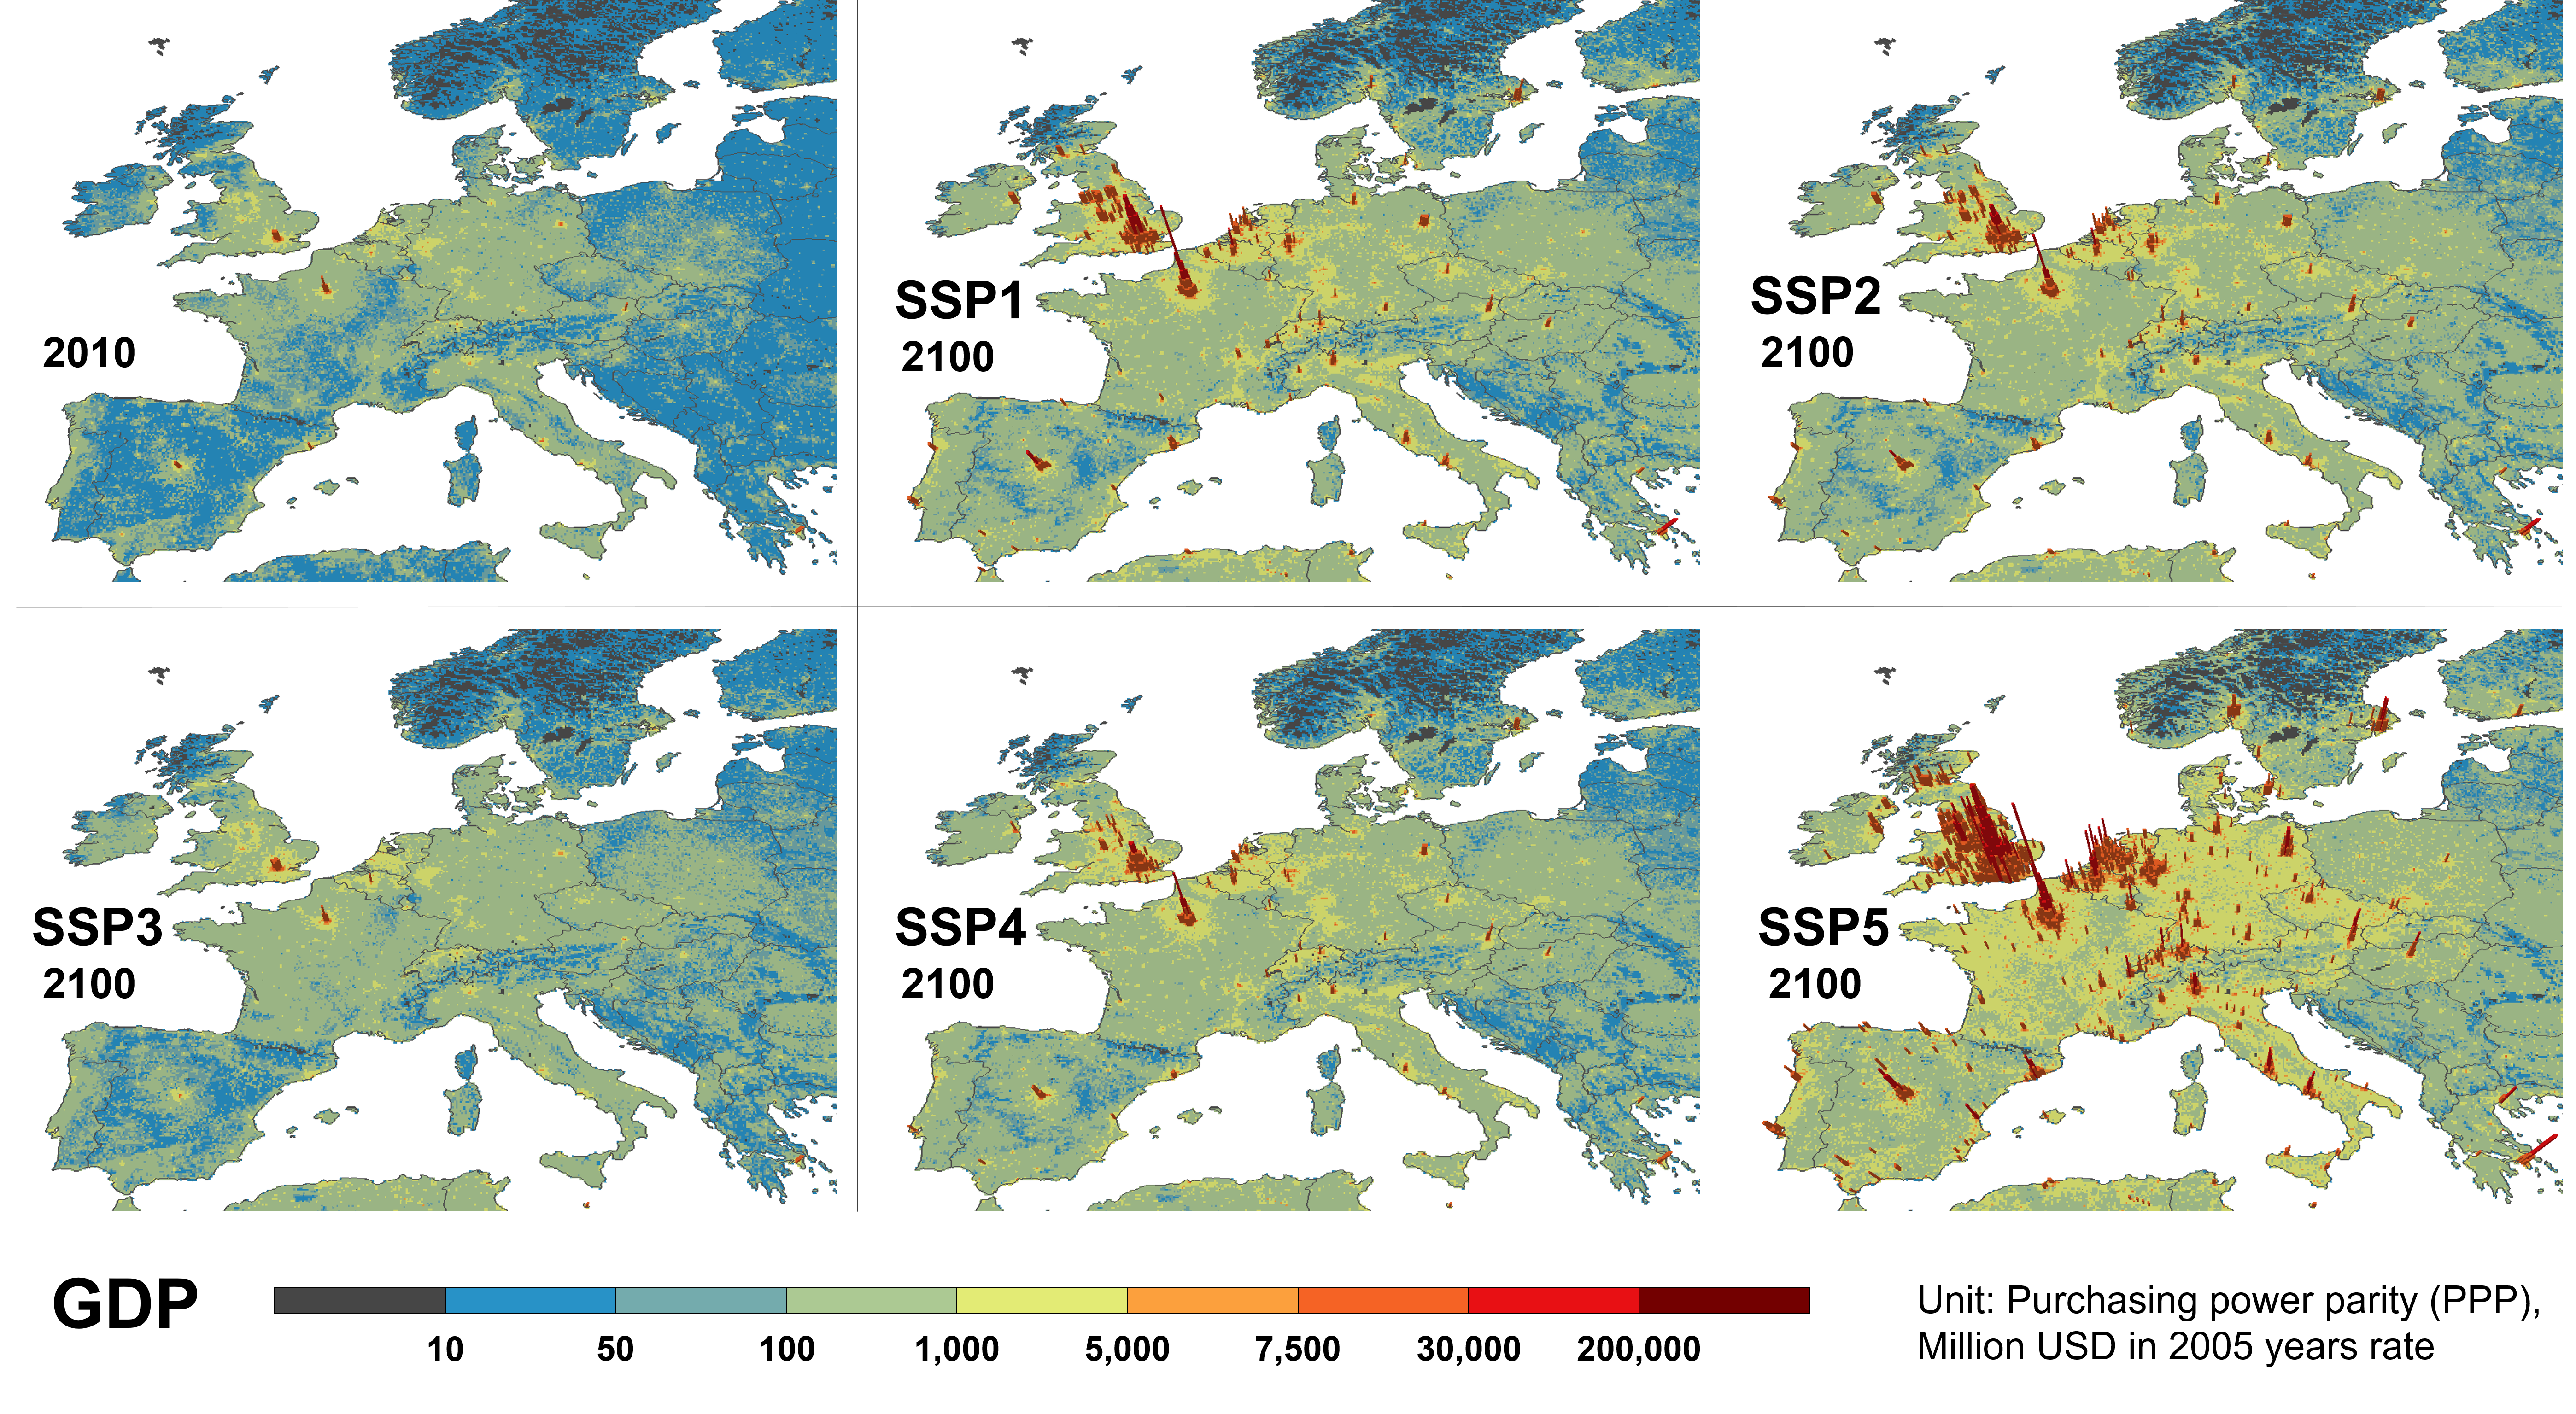
\includegraphics{Euro_2-5D.png}
\caption{Figure: Europe in 2.5D}
\end{figure}

\begin{figure}
\centering
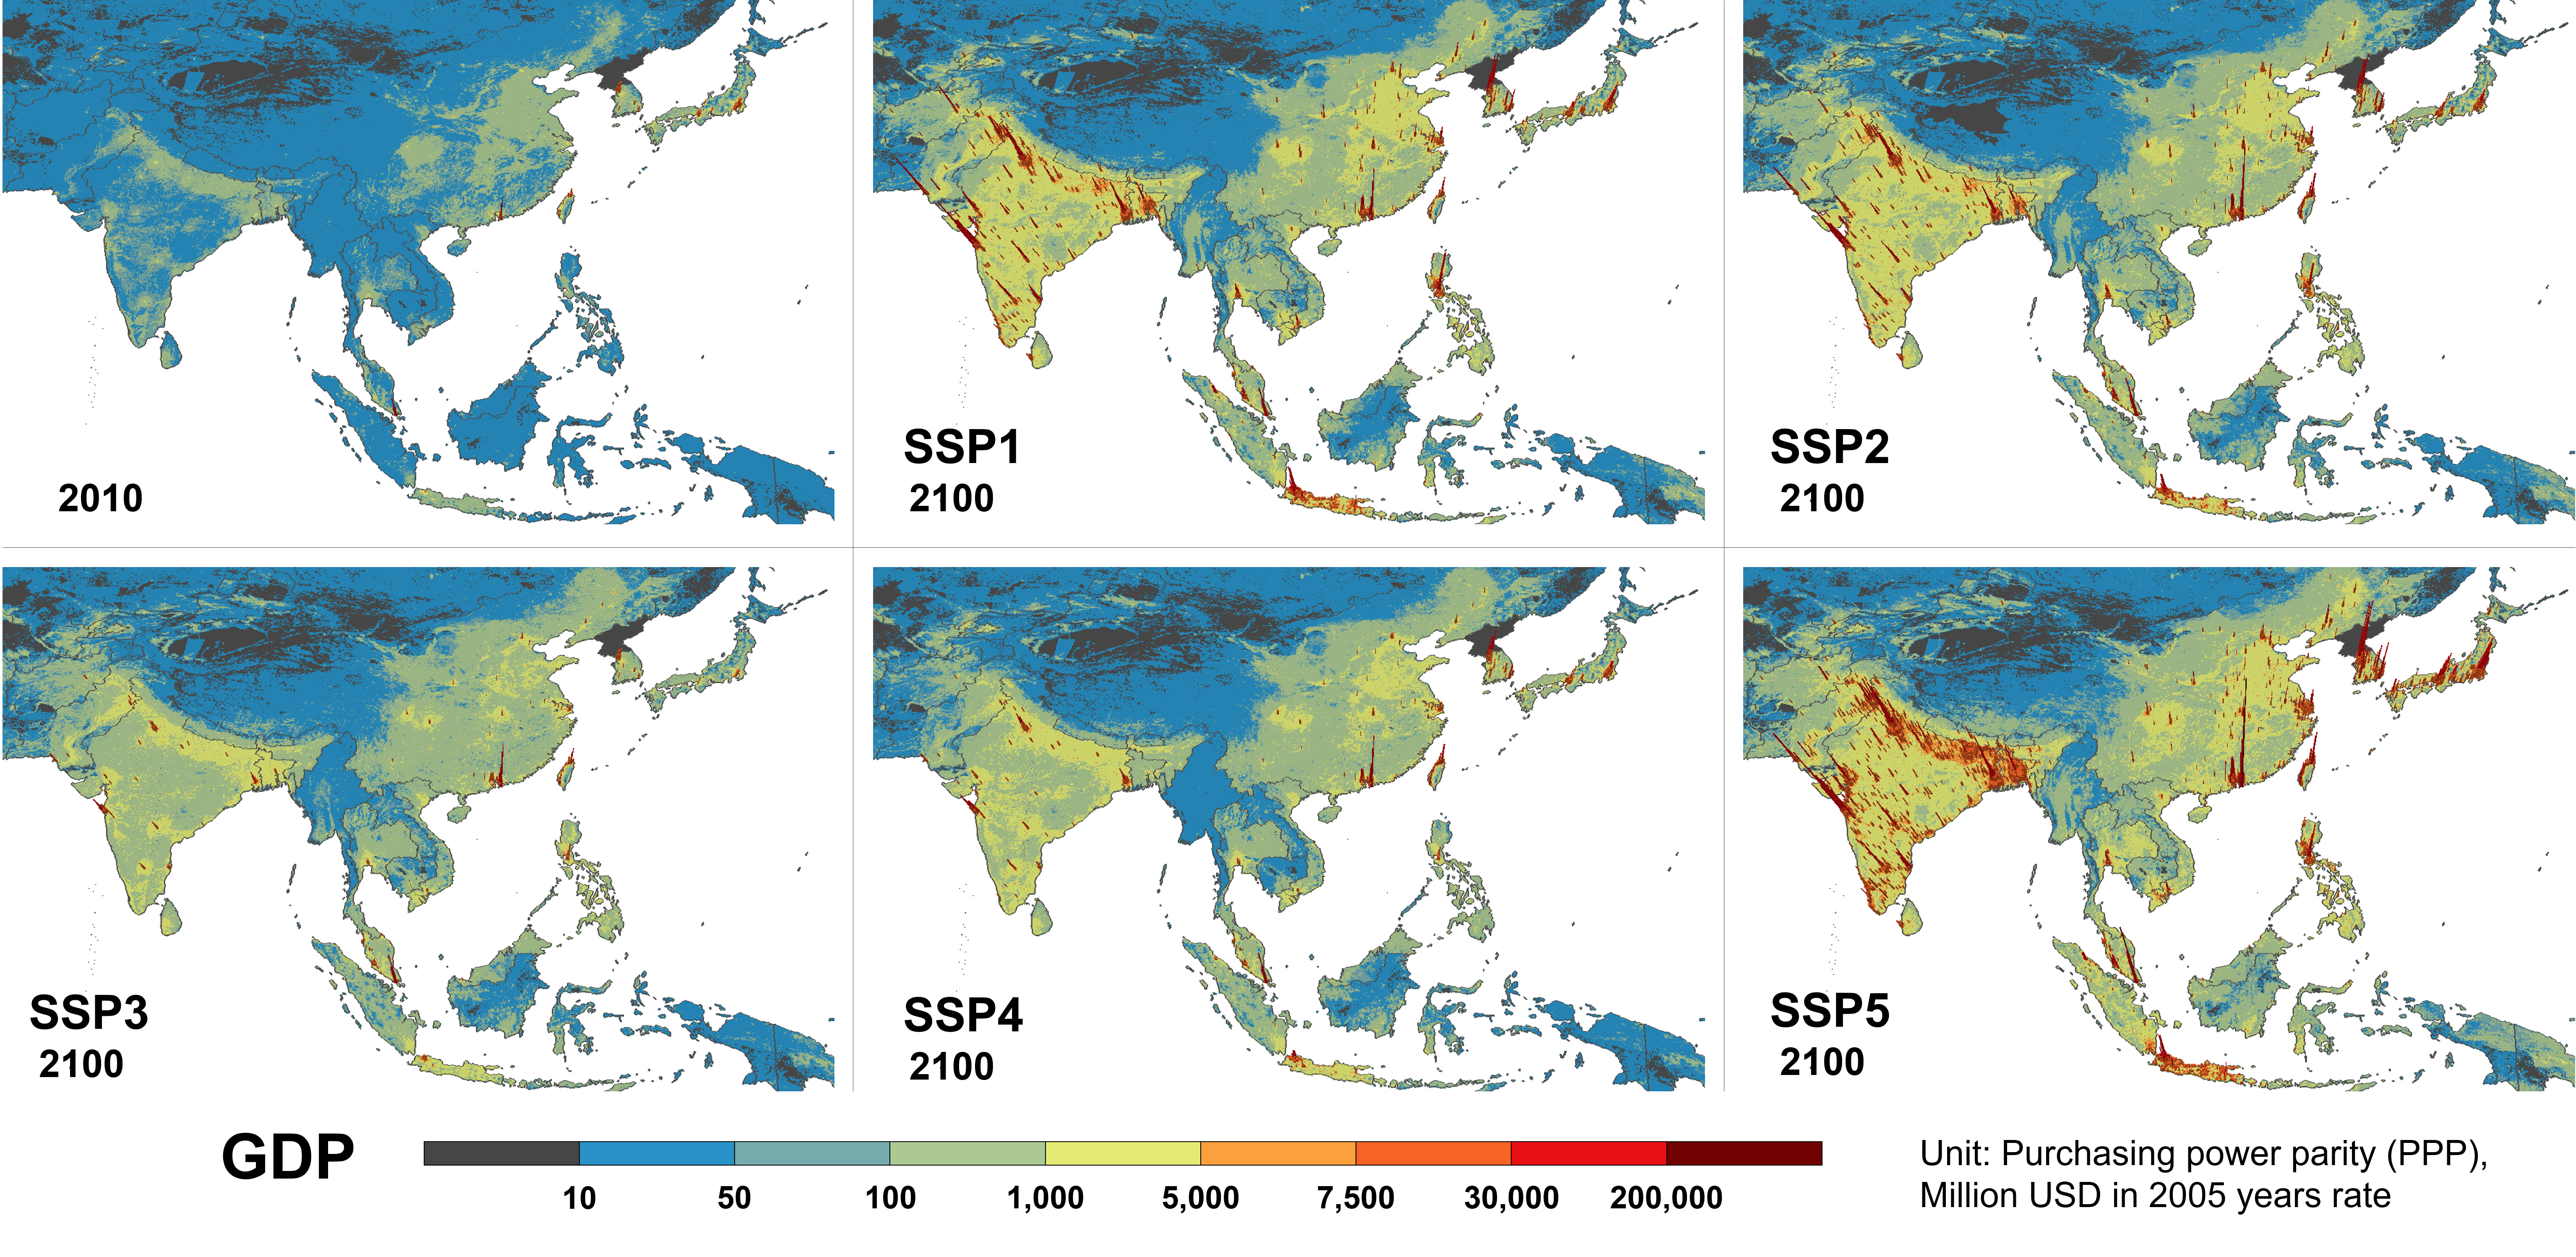
\includegraphics{Asia_2-5D.png}
\caption{Figure: Asia in 2.5D}
\end{figure}

\begin{verbatim}
## PhantomJS not found. You can install it with webshot::install_phantomjs(). If it is installed, please make sure the phantomjs executable can be found via the PATH variable.
\end{verbatim}

Figure: Interactive 3D globe maping on downscaled GDP. You can pan and zoom the globe by mouse-over.

\begin{center}\rule{0.5\linewidth}{0.5pt}\end{center}

\hypertarget{data-download}{%
\section*{Data download}\label{data-download}}
\addcontentsline{toc}{section}{Data download}

The GDPs for SSP 1--5 between 1850 and 2100 by 10 years are estimated by 2160 x 4320 grids, each of which are 1/12-degree grids, covering the globe. The GDP estimates in each year in each SSP are recorded as a GeoTIff image with resolution of 2160 x 4320. GeoTiff is a Tiff image with spatial coordinates for each grid cell; the coordinates are given by longitude and latitude measured by World Geodetic System 1984 (WGS84).

\textbf{\emph{GeoTiff}}: {[}\href{https://figshare.com/articles/dataset/Gridded_GDP_projections_compatible_with_the_five_SSPs_Shared_Socioeconomic_Pathways_/12016506/1}{please click here}{]}

\begin{center}\rule{0.5\linewidth}{0.5pt}\end{center}

\hypertarget{code-for-visualization}{%
\section*{Code for visualization}\label{code-for-visualization}}
\addcontentsline{toc}{section}{Code for visualization}

We used \href{https://www.r-project.org/}{\textbf{R}} for the 3D globe visualization.

\begin{verbatim}
## ------------------
## 3D visualization
## ------------------
library(colorRamps)
library(data.table)
library(dplyr)
library(htmlwidgets)
library(threejs)
library(tidyr)

setwd(****) # please set a directory including the file
dat <- data.table::fread(****) # please wait a moment!
# dat[1:3,]
#    longitude latitude gdp
# 1: -36.54172  83.5416   *
# 2: -36.45839  83.5416   *
# 3: -36.37506  83.5416   *

dat <- dat %>%
       dplyr::mutate(gdp=if_else(gdp>0,gdp,0)) %>%
       dplyr::filter(gdp>0) %>%
       dplyr::mutate(gdp.cut=as.numeric(cut(gdp,
        breaks=c(0,10^4,10^5,10^6,2.5*10^6,5.0*10^6,
                 10^7,2.5*10^7,5.0*10^7,10^8,10^9,max(gdp)), 
        include.lowest=TRUE))) %>%
       dplyr::mutate(pid=as.numeric(rownames(.))%%10) %>% # to avoid heavy calculation.
       dplyr::filter(pid==0)
3Dglobe <- threejs::globejs(lat=dat$latitude, long=dat$longitude,
        val=dat$gdp/10^6, # to adjust bar height 
        color=colorRamps::matlab.like(11)[dat$gdp.cut],
        pointsize=1.6,
        atmosphere=F)
3Dglobe        
\end{verbatim}

\begin{center}\rule{0.5\linewidth}{0.5pt}\end{center}

  \bibliography{book.bib,packages.bib}

\end{document}
